\chapter{Background}\label{chap:background}
\begin{overview}
  In this chapter, background information is presented on the commercial MPC software used. 
  Information regarding the case studies investigated, are also presented here.
\end{overview}

\section{Commercial MPCs}
The general concepts of MPCs have been discussed in section ~\ref{sec:mpclit}.
This section gives a more detailed overview of two popular commercial MPC packages.

Appendix~\ref{app:screenshots} contains screenshots of the interfaces mentioned in the sections that follow.

\subsection{Honeywell RMPCT}
Honeywell's MPC controller, RMPCT, forms part of their advanced process control suite, Profit Suite.
A brief overview of the controller and optimizer is given below. 
Attention is given to the controller internals as well as the interface used to build such a controller.
The information presented in this section is taken from \citet{honeywell1}, \citet{honeywell2} and \citet{honeywell3} unless stated otherwise.

\subsubsection{Models}
For the purpose of predictions, process models usually need to be identified first -- typically done via step testing.
\citet{honeywell3} lists the types of models which are supported by the Identifier and elaborates on their specific application.
These model types include;
\begin{itemize}
\item FIR,
\item PEM (the structure of which supports FIR, ARX, ARMA, ARMAX, ARIMA(X), ARARMAX, BJ and OE models) and
\item Laplace domain parametric models.
\end{itemize}
The final model, however, is saved in the Laplace domain.
Discrete models are converted to the {\it s} domain and has a final structure as shown in equation~\ref{eq:rmpctmodel}.
\begin{equation}
  \label{eq:rmpctmodel}
  G(s) = \frac{k(b_{n-1}s^{n-1}+ \cdots b_1s+1)e^{-ds}} {s(a_ns^n+a_{n-1}s^{n-1}+ \cdots a_1s+1)}
\end{equation}
The leading {\it s} in the denominator of equation~\ref{eq:rmpctmodel} indicates an integrator in any of the sub-processes.

If a third-party model exists, then the model converter in Profit Suite can be used to convert it into a suitable form.
  
\subsubsection{Constraints}
For MVs, the implementation of control constraints are in the form of high/low limits and movement limits.
The high/low limits of MVs are never violated.
Prioritisation and move suppression of MVs are done by means of weighting factors.
The movement load is spread across the MVs as per equation~\ref{eq:rmpctmvload},
\begin{equation}
  \label{eq:rmpctmvload}
  \min \sum_j \Delta u_j^2 \times weight_j^2
\end{equation}
where $j$ is the index of the MV.

CV control constraints are also specified as high/low limits.
In the event of negative degrees of freedom, constraints are prioritised by means of a give-up factor called the engineering unit (EU) give up.
Similar to equation~\ref{eq:rmpctmvload} the cumulative weighted error on the CVs are minimised as per equation~\ref{eq:rmpctcverror} with the $weight$ defined as shown and where $i$ is the CV index.
\begin{align}
  \label{eq:rmpctcverror}
  \min \sum_i weight_i^2 \times error_i^2 \\
  weight = \frac{1}{(\text{CV scaling factor})_i\sqrt{(\text{EU give up})_i}} \notag
\end{align}

The optimisation constraints are defined as being a specified amount within the high/low control limits.
These limits are not used for control.
For the constraining of dynamic response, funnels are implemented.
Predefined funnel types can be chosen from;
\begin{itemize}
\item Type 0, which is an automatically generated funnel,
\item Type 1, defined as a third of the Type 0 funnel pinched using the feedback performance ratio (FPR), and
\item Type 2, which is like Type 1 but pinched with the decouple ratio (Type 2 is therefore FPR independent).
\end{itemize}
Figure~\ref{fig:rmpctfunnel} illustrates the concept of pinching for the RMPCT funnels.
The definitions of the FPR and the decouple ratio are contained in \citet{honeywell1} but omitted from this dissertation.
\begin{figure}[htbp]
  \centering
  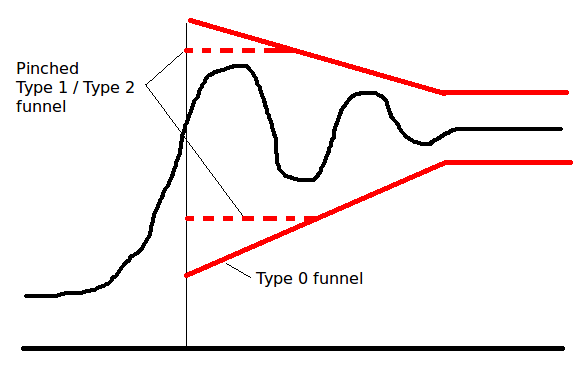
\includegraphics[width=8cm]{rmpct_funnel}
  \caption[RMPCT funnel implementation]{RMPCT funnel implementation showing pinched funnels with dashed lines.}
  \label{fig:rmpctfunnel}
\end{figure}

\subsubsection{Interface}
Profit Design Studio (figure~\ref{fig:ssrmpctmodel}) is used for model identification.
From this interface the process model can be extracted.
All the constraints (as discussed in the preceding section) can be added using this interface, where after the controller is built for on-line use from the Runtime Studio interface (figure~\ref{fig:ssrmpctcontrolbuild}).

The operator interface, Profit Suite Operator Station (figure~\ref{fig:ssrmpctoperator}), allows for constraint changes during plant operation.
As far as feasibility of constraints are concerned, these constraints are only checked to be within the Engineering limits (an additional constraint present in this interface).
A gain matrix (the steady-state model) can easily be obtained from this interface.

%screenshots?

\subsection{AspenTech DMCPlus}
Aspen Technologies' MPC controller, DMCPlus, forms part of their advanced process control suite, aspenONE.
The overview presented in this section is taken from \citet{aspentech1} unless stated otherwise.

\subsubsection{Models}
Model identification is done with DMCplus Model or with SmartStep which enables model identification whilst still maintaining control of a plant.
Models are stored as FIR models and conversion to and from other model types are not supported.
Extracting a steady-state gain matrix is however possible as the gains are displayed during the modelling phase.

\subsubsection{Constraints}
As with RMPCT, constraints on the CVs and MVs are specified as high/low limits.
In addition to the constraints, equal concern errors (ECEs) are used to calculate the optimal move plan and emphasise the relative importance of CVs.

Three types of constraints are used;
\begin{itemize}
\item Validity limits which describe limits on measured variables and the values they can attain.
These are the outermost limits.
\item Engineering limits are the hard limits in which the process is operated and are not violated in a solution.
The engineering limits lie within the validity limits.
\item Operator limits are used for optimisation, with successful solutions keeping to these limits.
These are the innermost limits, contained within the engineering limits.
\end{itemize}

For constraint handling, rank groups are used.
Constraints are ranked and lower rank constraints are considered ``hard'' whereas higher ranking constraints are relaxed until steady-state feasibility is achieved.
Optimisation constraints are ranked at 1000 and constraints that are ignored are ranked at 9999.

The constraint handling of integrating variables is done by utilising ramp rates.
Constraints on the variable is generated using a factor of the time to steady-state and the upper and lower bound.
This limits the rate of change of a variable.
Figure~\ref{fig:dmcplusramprates} shows the constraints generated using ramp rates.
Note that the 'inverted funnel' becomes sharper when a the full time to steady-state is used as opposed to a fraction thereof.

\begin{figure}[htbp]
  \centering
    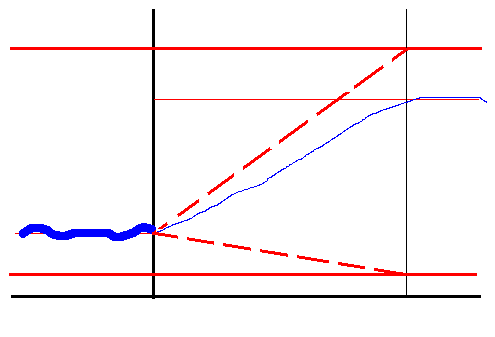
\includegraphics[width=8cm]{graph/dmcplusramprate}
  \caption[DMCPlus ramp rate dynamic constraints]{Ramp rates creating dynamic constraints on integrating variables.}
  \label{fig:dmcplusramprates}
\end{figure}

\subsubsection{Interface}
The DMCPlus Model (figure~\ref{fig:ssdmcplusmodel}) interface is used to obtain models from data.
Obtaining a gain matrix is possible from this interface.
Additions to the model matrix is also done from this interface.

The controller is built using the DMCPlus Build interface (figure~\ref{fig:ssdmcpluscontrolbuild}).
Models obtained in the previous step is implemented and a configuration file for the controller generated.

The Production Control Web Interface (figure~\ref{fig:ssdmcplusoperator}) is used by operators to interact with the process.
This interface is used to actively change constraints on inputs and outputs.

\section{Case studies}
The following actual systems were investigated to test the method, proposed in chapter~\ref{chap:conhand}.
All rigs investigated are from the Process Modelling and Control laboratory of the University of Pretoria.

\subsection{Level and flow rig}
\subsubsection{System description}
The level and flow rig consists of two control valves, a measured flow (to one control valve) and a measured level.
Figure~\ref{fig:flowphoto} shows the rig along with its process flow diagram.
\begin{figure}[htbp]
  \centering
    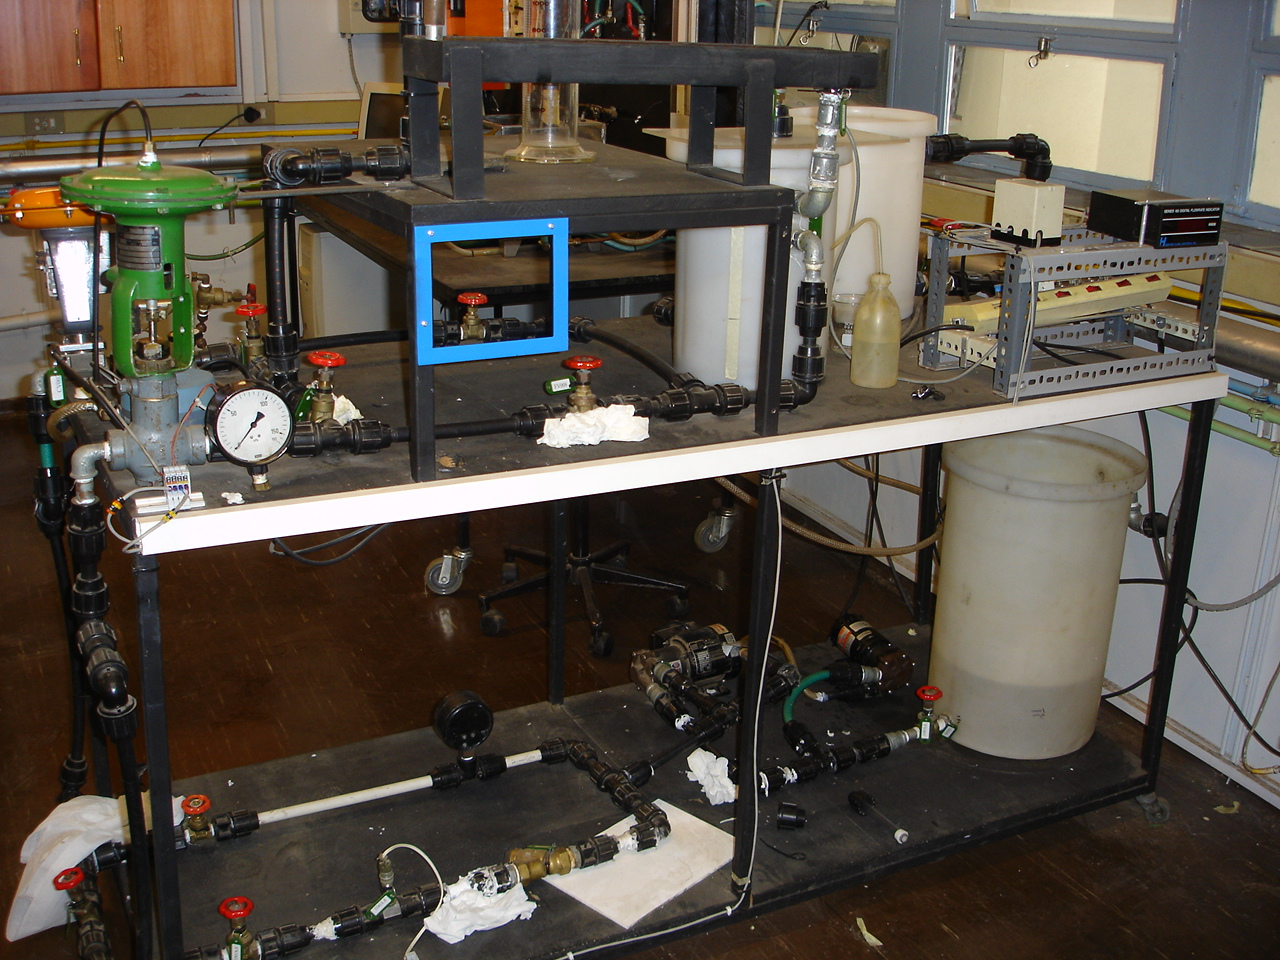
\includegraphics[width=7cm]{graph/flowphoto.JPG}
    \qquad
    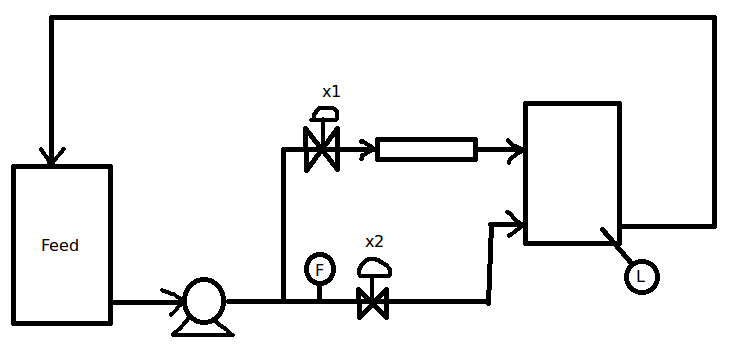
\includegraphics[width=7cm]{graph/flowpfd}
  \caption[Level and flow rig photo and flow diagram]{Level and flow rig photo (left) and process flow diagram (right).}
  \label{fig:flowphoto}
\end{figure}

\subsubsection{Process model}
The level and flow rig is modelled as a $2\times2$ system.
The MVs are the milliamp signals sent to the valves ($x_1\text{ \& }x_2$).
These signals correspond to the opening fractions of the two valves.
The CVs are the flow ($F$) and the level ($L$).
The steady-state gain matrix of this process is shown in equation~\ref{eq:flowmodel}.
Note that valve 1 is an air-to-close valve and valve 2 is an air-to-open valve, which explain the negative gain in element 1 of $G_{fl}$.
\begin{equation}
  \label{eq:flowmodel}
                    %x1       x2
    G_{fl} = \bpm -0.0476 & -0.0498 \\      %L
                  0.0111 & -0.0604 \\ \epm %F
\end{equation}
\subsubsection{Operating conditions}
The operating conditions for this rig is shown in table~\ref{tab:flowopcon}
\begin{table}[htbp]
  \centering
  \begin{tabular}{llllll}
    \toprule
    \multicolumn{2}{c}{Variable} & \multicolumn{2}{c}{Operating range} & \multicolumn{2}{c}{Physical constraints} \\
    && Low & High & Low & High \\ 
    \midrule
    Inputs &$x_1 (\text{mA})$ & 4 & 20 & 4 & 20 \\
           &$x_2 (\text{mA})$ & 4 & 20 & 4 & 20 \\[1.3ex]
    Outputs &$F~(\text{gpm})$ & 1.2 & 1.5 & 0 & 1.9 \\
            &$L~(\text{cm})$  & 15 & 18 & 6 & 25 \\
    \bottomrule
  \end{tabular}
  \caption{Operating conditions of level and flow rig.}
  \label{tab:flowopcon}
\end{table}

\subsection{Laboratory distillation column}
\subsubsection{System description}
The second case study considered is a 10-plate distillation column.
The column is run as a closed system with bottoms and distillate mixed and fed back into the column.
Figure~\ref{fig:columnphoto} shows a photo of the column along with its process flow diagram.
\begin{figure}[htbp]
  \centering
    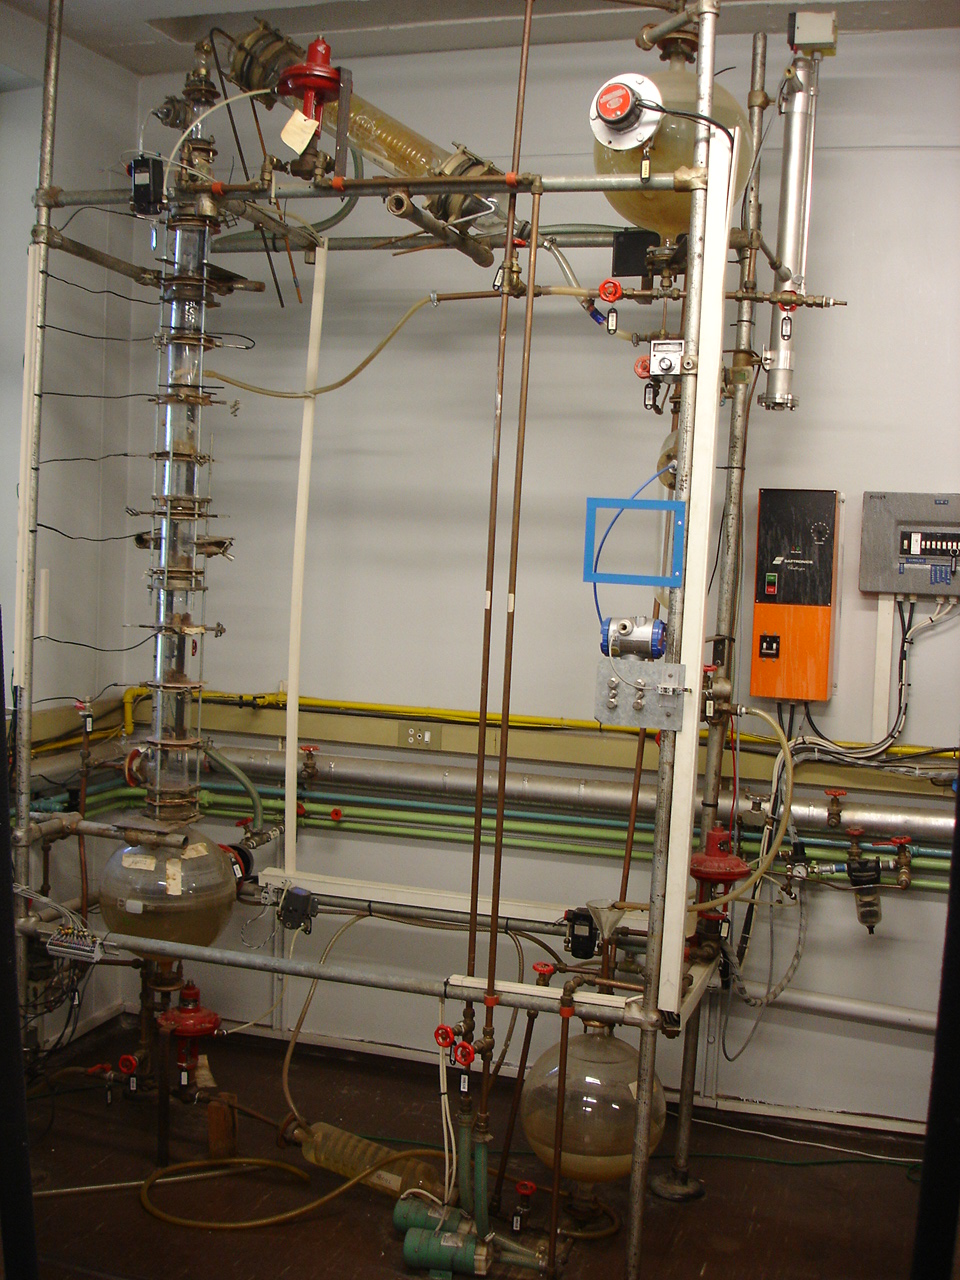
\includegraphics[width=7cm]{graph/columnphoto}
    \qquad
    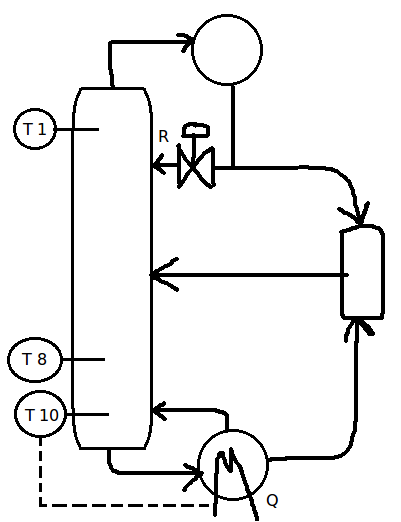
\includegraphics[width=7cm]{graph/columnpfd}
  \caption[Laboratory distillation column photo and flow diagram]{Laboratory distillation column photo (left) and flow diagram (right).}
  \label{fig:columnphoto}
\end{figure}

\subsubsection{System model}
The process model has been reduced to a $2\times2$ matrix.
Reflux flowrate ($R$) and the setpoint of plate 10's temperature ($T_{10~sp}$) are the MVs, and the temperatures of plate 1 and 8 ($T_1\text{ \& }T_{8}$) are the CVs.
The input to the model for $R$ is a milliamp value sent to the valve.
Figure~\ref{fig:columnmodel} shows a graphic representation of the column model and equation~\ref{eq:columnmodel} gives the values of the steady-state gain model.
\begin{equation}
  \label{eq:columnmodel}
                 % R      T10sp
  G_{col} = \bpm -0.0575 & 0.96 \\       % T1
                -0.146  & 0.518 \\ \epm % T8
\end{equation}
\begin{figure}[htbp]
  \centering
    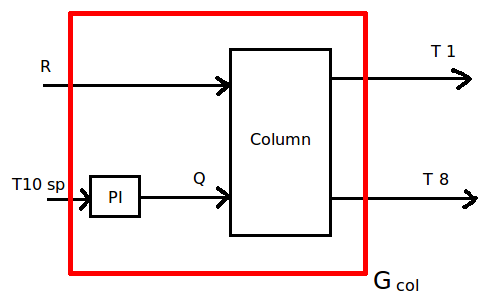
\includegraphics[width=8cm]{graph/columnmodel}
  \caption[Column model]{Column model showing internal PI controller.}
  \label{fig:columnmodel}
\end{figure}

The PI controller between $T_{10~sp}$ and $Q$ was added as a safety measure, should the advanced control layer fail.

\subsubsection{Operating conditions}
Table~\ref{tab:columnopcon} shows the operating conditions of the distillation column.
\begin{table}[htbp]
  \centering
  \begin{tabular}{llllll}
    \toprule
    \multicolumn{2}{c}{Variable} & \multicolumn{2}{c}{Operating range} & \multicolumn{2}{c}{Physical constraints} \\
    && Low & High & Low & High \\ 
    \midrule
    Inputs &$R~(\text{mA})$          & 11 & 15 & 4 & 20 \\
           &$T_{10~sp}~(\degrees{C})$ & 78 & 82 & 0 & 90 \\[1.3ex]
    Outputs &$T_1~(\degrees{C})$     & 66 & 68 & 15 & 68 \\
            &$T_{8}~(\degrees{C})$   & 78 & 82 & 25 & 90 \\
    \bottomrule
  \end{tabular}
  \caption{Operating conditions of distillation column.}
  \label{tab:columnopcon}
\end{table}

% Local Variables:
% TeX-master: "AHC_thesis"
% End: